\section{\gls{mfms}}
\label{sec:mfms}
    This section will explain \gls{mfms} in greater detail.
    Akin to other fingerprinting-based radiolocation systems, \gls{mfms} consists of two main phases.
    During the offline phase, \gls{rss} information from anchor nodes is collected at many locations in the environment and used to approximate the radio wave propagation function.
    The online phase, on the otherhand, makes use of the approximated propagation function obtained in the former phase.
    %  is used for localization purposes with new observations obtained at arbitrary locations.
    However, one major difference between \gls{mfms} and conventional approaches is that \gls{mfms} employs three different sources of information to infer the location of the agent.
    The main motivation behind employing multisource information is to exploit the diversity of the propagation characteristics of the different frequencies.

    \begin{figure}[thpb]
       \centering
       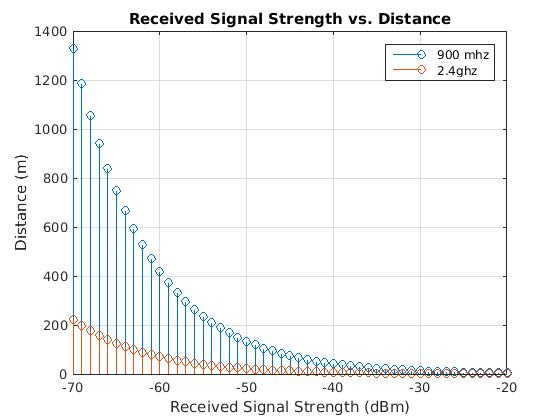
\includegraphics[width=\linewidth]{figures/rss-vs-distance.jpg}
       \caption{\label{fig:log-distance}RSSI readings of NLoS and LoS APs acquired with a stationary agent}
    \end{figure}

    As it can be seen in the \Cref{eq:log-distance} and \Cref{fig:log-distance}, the received power and separation distance has a log-linear relationship.
    %  demonstrates the log-distance relationship between received power and the separation between two antennas in two different frequencies in \gls{uhf} radio band.
    This figure implies two fundamental problems in radiolocationing systems:
    The first problem is that as the carrier frequency increases path loss increases significantly, which limits the radio covarage and localization ability of the system in large environments.
    On the other hand, as the carrier frequency increases, the separation between two antennas, i.e.\ the anchor node and the target to be localized, can be identified with finer spatial resolution.
    Therefore, the trade-off between radio coverage and spatial localization resolution can be resolved by employing different frequencies in indoor localization systems by fusing the information acquired from the anchor nodes using different carrier frequency.

    \Cref{fig:module} shows the outline of the \gls{mfms} in the hardware scope.
    In order to achieve wider spatial coverage, \gls{mfms} employs XBees working at 900 MHz.
    On the other hand, finer spatial resolution accomplishment is achieved by ESP32 modules which runs at 2.4 GHz WiFi and Bluetooth.
    In other words, each anchor node contains an XBee working at 900 MHz and an ESP32 module working at 2.4 GHz WiFi and Bluetooth.

    \begin{figure}[thpb]
       \centering
       
\includegraphics[width=\linewidth]{figures/placeholder.png}
       \caption{\label{fig:module}\gls{mfms} Anchor Nodes}
    \end{figure}

    \subsection{Offline Phase}

        \subsubsection{Data Acquisition}

        \subsubsection{Training}

    \subsection{Online Phase}

        \subsubsection{Inference}

        \subsubsection{Information Fusion}
